Una parte necesaria para entender la capa física del modelo OSI es el de los tipos de medios de transmisión de datos, en este caso haré un vistazo a los \textit{Medios de Transmisión Guiados.} 
Para comenzar hay que recordar que el medio en un sistema de transmisión de datos, es la ruta física entre el transmisor y el receptor. Con esta definición podemos decir que un \textbf{medio de transmisión guiado} es llamado así debido a que la señal que viaja a través de cualquiera de estos medios está dirigida y contenida por los límites físicos del medio.
\section{Tipos de Medios de Transmisión Guiados}
En general hay 3 tipos de medios guiados (Data Communications And Networking 4th Edition, Behrouz A. Forouzan): \\
\begin{center}
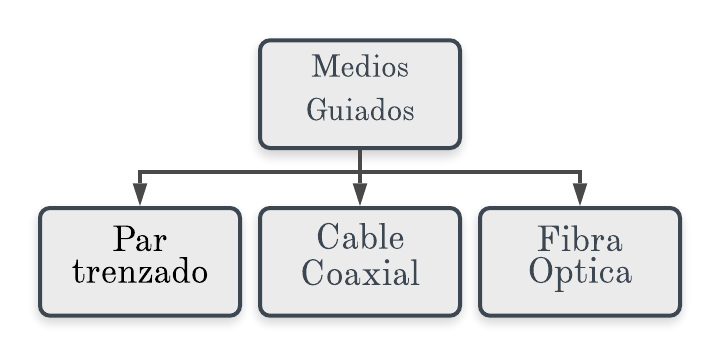
\includegraphics[scale=0.25]{D1}
\end{center}
\subsection{Par Trenzado}
Este es el medio de transmisión menos costoso y mas utilizado.
\subsubsection{Descripción Física}
Un par trenzado consta de dos alambres de cobre aislados dispuestos en un patrón espiral regular.  Por lo general, varios de estos pares se agrupan en un cable envolviéndolos en una cubierta protectora resistente. En distancias más largas, los cables pueden contener cientos de pares.
\begin{figure}[!ht]
\centering
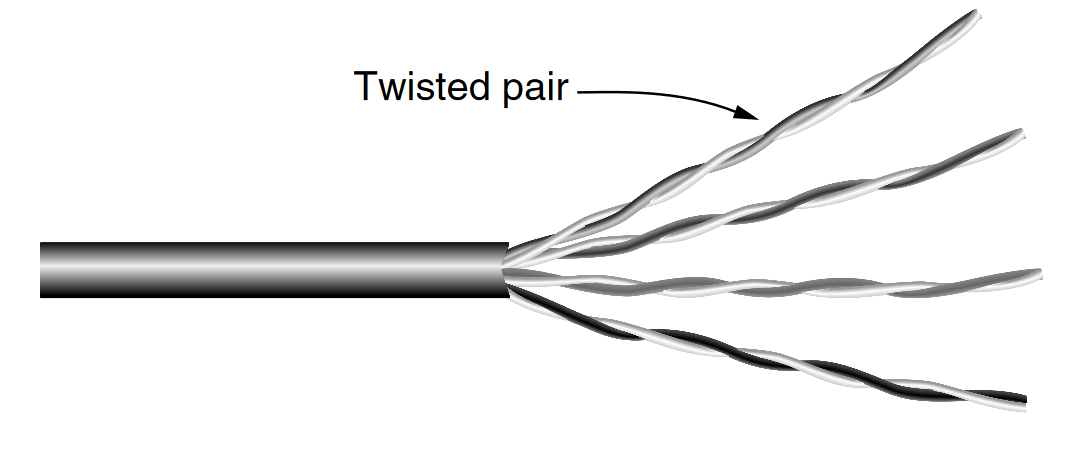
\includegraphics[scale=0.5]{D2}
\caption{Cable \texttt{UTP} con cuatro pares trenzados.}
\end{figure}
\subsubsection{Aplicaciones}
Es el medio de transmisión más común para señales analógicas y digitales ademas es utilizado en la red telefónica y también se usa comúnmente dentro de edificios para redes locales que admiten computadoras personales.
\subsection{Cable Coaxial}
\subsubsection{Descripción Física}
El cable coaxial, como el par trenzado, consta de dos conductores, pero está construido de manera diferente para permitirle operar en un rango más amplio de frecuencias. Consiste en un conductor cilíndrico exterior que se encuentra debajo de un único conductor de cable interno.
\begin{figure}[!ht]
\centering
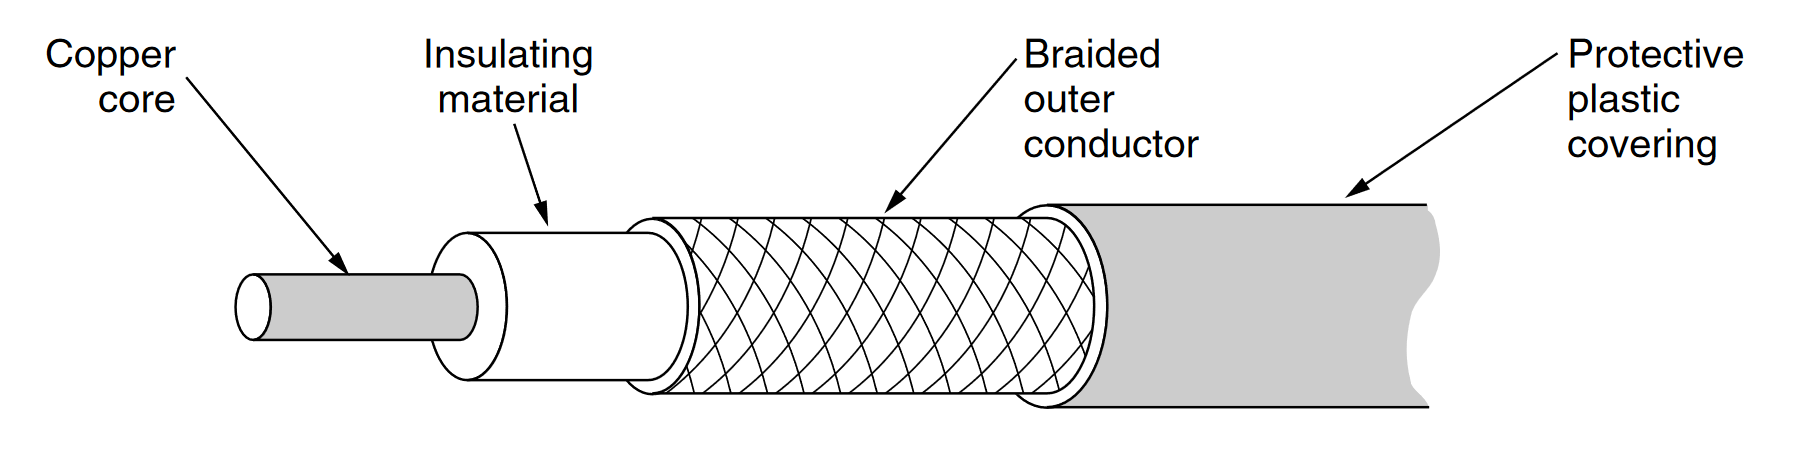
\includegraphics[scale=0.45]{D3}
\caption{Cable Coaxial}
\end{figure}
\subsection{Fibra Óptica}
\begin{figure}[!ht]
\centering
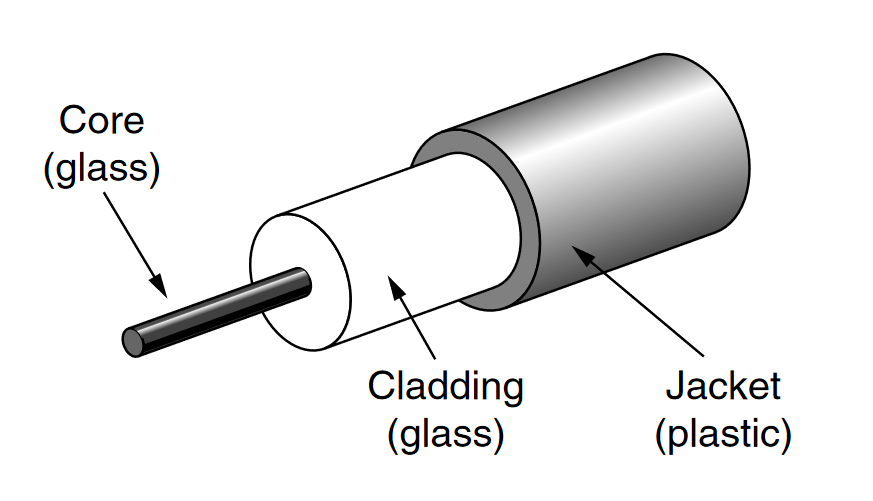
\includegraphics[scale=0.45]{D4}
\caption{Una sola fibra.}
\end{figure}